\documentclass[11pt]{article}
\usepackage[top=2.5cm, bottom=2.5cm, left=2cm, right=2cm]{geometry}
\usepackage[utf8]{inputenc}
\usepackage[icelandic]{babel}
\usepackage[T1]{fontenc}
\usepackage[sc]{mathpazo}
\usepackage[parfill]{parskip}
\usepackage{booktabs}
\usepackage{amsmath}
\usepackage{color}
\usepackage{graphicx}
\usepackage{wrapfig}
\usepackage{subcaption}
\usepackage{minted}
\usepackage{multicol}
\usepackage{lipsum}
\usepackage[pdftex,bookmarks=true,colorlinks=true,linkcolor=blue,urlcolor=blue, citecolor=blue]{hyperref}
\usepackage[all]{hypcap}

\hyphenpenalty=9000

\newcommand{\matlab}[1]{\inputminted[linenos, frame=lines, label=#1, fontsize=\small]{matlab}{#1}}
\renewcommand{\listingscaption}{Kóði}

% One-column environment definitons for multicol - not floating!
\makeatletter
\newenvironment{tableonecolumn}{\begin{minipage}{\linewidth}\begin{center}\def\@captype{table}}{\end{center}\end{minipage}}

\newenvironment{figureonecolumn}{\begin{minipage}{\linewidth}\begin{center}\def\@captype{figure}}{\end{center}\end{minipage}}
\makeatother

\title{Framleiðsla á humulene í Saccharomyces cerevisiae}
\author{Eiríkur Ernir Þorsteinsson \and Jónas Tryggvi Stefánsson}
\date{}

\begin{document}

\maketitle

\setlength{\columnsep}{1cm}

\begin{abstract}
Fjallað er um framleiðslu á humulene, efnasambandi sem finnst í humlum. Markmiðið var að finna lausn á Humulene-framleiðslu í massavís eða samhliða klassísku bjór-bruggferli. Notast var við Matlab, COBRA Toolbox, CVX og Gurobi.  OptStrain reikniritið m.t.t. Yeast 7 gersvepps-líkansins var svo útfært  til þess að finna æskilega lausn á því að hámarka framleiðslu á humulene. Niðurstöðurnar voru þær að það er hægt að örva framleiðsluna með útslætti. Samanburður á framleiðslu fyrir og eftir útslátt leiddi í ljós að vöxturinn jókst ekki nógu mikið til þess að framleiðsla í massavís myndi borga sig. Hinsvegar kom í ljós að framleiðsla á humulene ein og sér í gersvepp við hefðbundið bjórgerðarferli er vænleg. Rannsóknir á viðfangsefninu með því að nota OptForce reikniritið, í stað OptStrain, væru áhugaverðar, það hefur gefið góða raun í sambærilegum verkefnum. Áhugavert sambærilegt verkefni væri að skoða Myrcene, mögulega mikilvægasta sesquitepene-ið þegar kemur að lykt bjórs.
\end{abstract}

\vspace{1cm}
\begin{multicols}{2}

% Myndir verða mikilvægar, fá 2-4
% Byrja á myndunum!
% Hugmynd: Flæðirit yfir virkni reikniritsins
\section{Inngangur}
Áfengi drykkurinn bjór ætti að vera flestum lesendum kunnugur. Hefðbundinn bjór er myndaður með gerjun á vatnsblönduðu korni og bragðbættur með humlum.

Humlar eru dýrt hráefni sem erfitt er að rækta á mörgum svæðum heimsins og hrörna hratt við geymslu. Þetta gefur ástæðu til að athuga hvort að hægt sé að minnka það magn humla sem bjórgerðin þarf með efnaviðbótum.

Humulene\cite[KEGG: C09684]{Kanehisa01012000} er eitt mikilvægra efnasambanda í lykt og bragði bjórs \cite{howard1957evaluation}. Lagt er upp með athuga reikningslegar forsendur fyrir því að nota erfðabreyttan gersvepp til að framleiða humulene, en þó nokkur fordæmi eru fyrir því að erfðabreyta gersveppum til nota í matvælaiðnaði \cite{dequin2001potential}.

Fyrirsjáanlegar eru tvær aðalleiðir til að hagnýta framleiðslu á humulene í gersvepp. Fyrri leiðin er að nota erfðabreyttan gersvepp til að gerja bjór í annars hefðbundnu bjórgerðarferli, svo framleiðslan á humulene væri samhliða framleiðslu á efnum á borð við etanól sem ávallt er að finna í bjór. Seinni leiðin er að besta framleiðslu á hreinu humulene, sem síðan væri einangrað og bætt út bjór gerjuðum með hefðbundnu geri.

Báðar hagnýtingarleiðir verða hér kannaðar með því að setja þær upp sem línuleg bestunarverkefni, en línuleg bestunarlíkön hafa verið notuð með góðum árangri til spá fyrir um möguleg efnaskiptaferli í örverum \cite{banga2008optimization,edwards2001silico}.
\section{Aðferð}
Línulegu bestunarverkefnin voru sett upp í Matlab. Þau voru leyst með aðstoð COBRA Toolbox, CVX og Gurobi.

Áskoranirnar sem felast í því að kanna leiðirnar tvær, humulene-framleiðslu í hefðbundnu bjórgerjunarferli og í ``efnaverksmiðju'' eru nokkuð mismunandi, en báðar leiðir byggjast á greiningu á líkani af gersveppnum.
\subsection{Líkan}
Notast var við Yeast 7 líkanið\cite{yeastsf} af \emph{Saccharomyces cerevisiae S288c}. Líkanið var valið vegna þess að það er umfangsmikið (m.t.t. fjölda gena og efnahvarfa), með lágt hlutfall blokkaðra efnahvarfa og lágt hlutfall dead-end efna. Önnur líkön gefa betri niðurstöður í sérhæfðum aðstæðum, en þessir eiginleikar Yeast 7 þóttu líklegir til að stuðla að nothæfum niðurstöðum í fyrstu hermunum \cite{heavner2015comparative}. 
\subsubsection{Viðbætur á líkani}
Þekkt ensím, (2E,6E)-farnesyl-diphosphate diphosphate-lyase, myndar humulene út frá farnesyl-diphosphate \cite[KEGG: R08373]{Kanehisa01012000}. Farnesyl-diphosphate finnst í terpenoid lífefnasmíðaferlinu \cite[KEGG: rn00900]{Kanehisa01012000}, en bestun á því efnaferli hefur fengið nokkra athygli \cite{BIT:BIT21216,misawa2011pathway,asadollahi2008production}.

Tveimur grundvallar-efnahvörfum var bætt við líkanið til að framleiða humulene úr farnesyl-diphosphate.
Um er að ræða efnahvarf sem framleiðir humulene úr farnesyl-diphosphate annars vegar og exchange-hvarf fyrir humulene-ið hins vegar. Þennan viðbætta ``pathway'' má sjá á mynd \ref{fig:pathway}.

\begin{figureonecolumn}
\caption[Viðbætur við Yeast 7]{Efnahvörf sem bætt var við Yeast 7 líkanið.}
\label{fig:pathway}
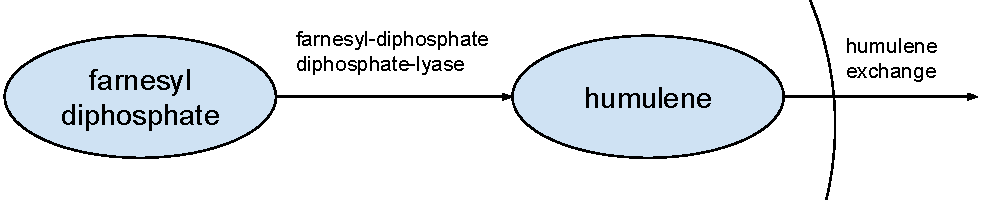
\includegraphics[width=\linewidth]{Pics/HumuleneAddition}
\end{figureonecolumn}
\begin{figure*}[b]
\caption[OptStrain reikniritið]{Skref OptStrain reikniritsins sem lýst er í \ref{sec:optstrain}. Sjá sérstakar viðbætur á mynd \ref{fig:pathway}}
\label{fig:flaedirit}
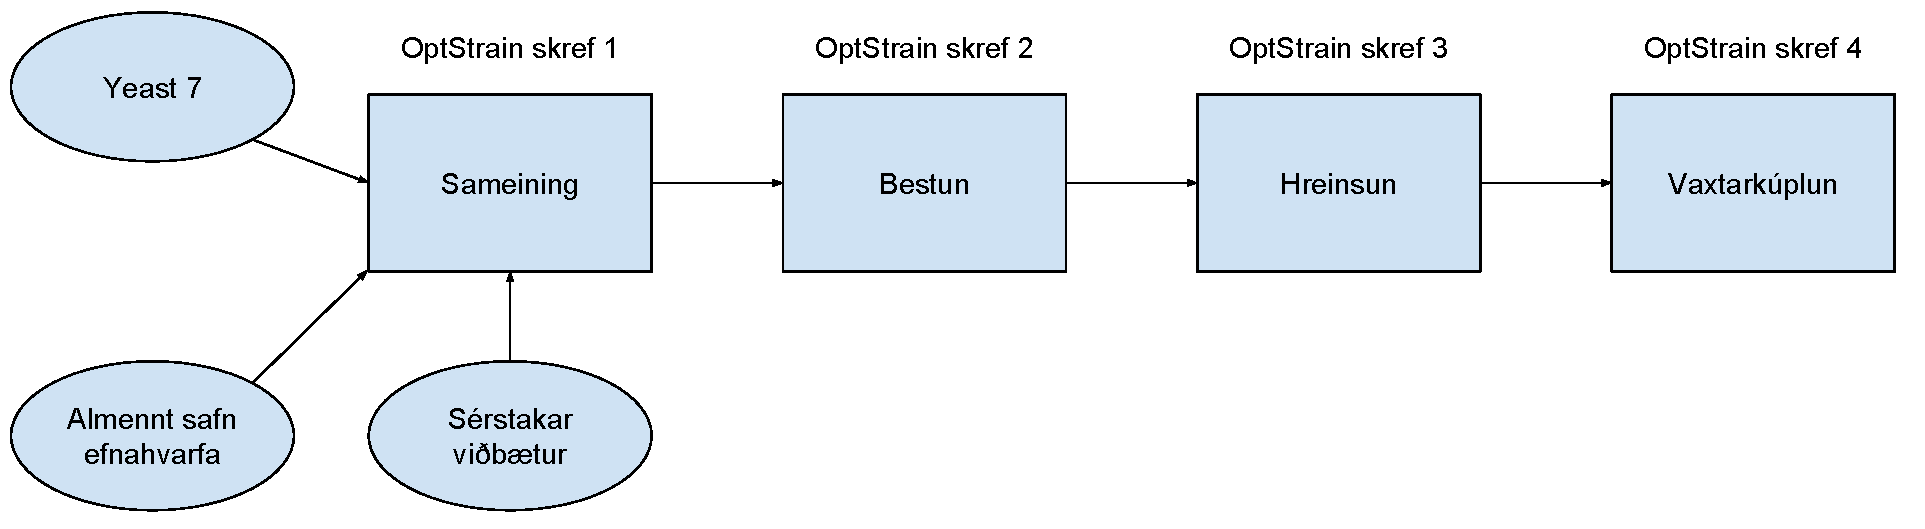
\includegraphics[width=\linewidth]{Pics/OptStrainOverview}
\end{figure*}
\subsection{Framleiðsla í hefðbundnu gerjunarferli}
\label{sec:hefdbundid}
Í hefðbundinni bjórgerð er svokallaður virtur fyrst framleiddur úr vatni og korni. Virturinn er sykruríkur vökvi sem síðar er gerjaður. Eiginleikar virtsins og aðstæður gerjunarinnar setja skorður á framleiðslu á humulene með þessari aðferð.
\subsubsection{Kolefnisgjafar og gefin skilyrði}
Gerjanlegu sykrurnar í virti eru frúktósi, glúkósi, súkrósi, maltósi og maltótríósi. Þar vega mest hlutverk maltósa, frúktósa og maltótríósa. Maltótríósi er ekki til staðar í Yeast 7 líkaninu og hlutverk annarra kolefnisgjafa er óverulegt, svo til einföldunar voru einungis maltósi og glúkósi tekin til skoðunar. Valin hlutföll eru 1 hlutur glúkósa á móti 2 hlutum maltósa, sem er nálægt meðalhlutföllum þeirra í virti \cite{otter1967determination}. 

Í bjórgerð fer gerjun að mestu leyti fram við loftfirrtar aðstæður. \emph{S. cerevisiae} getur vaxið við slík skilyrði \cite{ishtar2007factors}, en líkanið nær ekki til þeirra.
\subsubsection{Markfall}
Þar sem framleiða á heildstæða vöru til neyslu er nauðsynlegt að stýra framleiðslu á fleiri efnum en einungis humulene. Mikilvæg efni í bjór \cite{dequin2001potential} sem tekin voru til athugunar eru:
\begin{itemize}
 \item etanól
 \item ísóamýl acetat, ábyrgt fyrir ``bananalykt'' af ýmsum gerðum bjórs
 \item glýseról, veitir sætutilfinningu
 \item þvagefni, sem ólykt er af og þarf að lágmarka
\end{itemize}
Markfall var smíðað sem tekur tillit til þessara efna. 

Æskilegu efnunum var úthlutað stuðlum sem jafna forgang þeirra m.t.t. fjölda kolefnisfrumeinda í efnunum, til að koma í veg fyrir að Cobra úthluti efnahvörfum sem seyta efnum með fáum kolefnisfrumeindum óeðlilega miklu flæði. ``Rétt'' gildi á þessum efnum myndi fara eftir gerð bjórsins sem framleiða ætti. Þetta er gert í kóðadæmi \ref{code:constructObjectiveFunction}.

\subsubsection{Útreikningar}
Flæðigreining (e. \emph{flux variability analysis}) og greining á þoli (e. \emph{robustness analysis}) voru framkvæmd á líkaninu. Þetta er gert í kóðadæmi \ref{code:enhancedBrewing}.

\subsection{Sérstök framleiðsla á humulene}
Sé ætlunin eingöngu að framleiða humulene óháð öðrum skilyrðum sem til staðar eru í bjór opnast fleiri möguleikar. Hér var sú leið farin að nota útgáfu af OptStrain reikniritinu \cite{pharkya2004optstrain} til að finna endurbætta útgáfu af gersveppnum.
\subsubsection{Skilyrði og markfall}
Einungis þarf að taka tillit til humulene-framleiðslu við þessar aðstæður, svo markfallið er einfaldara. Blanda maltósa og glúkósa var áfram notuð sem kolefnisgjafi til að auðvelda samanburð við framleiðslu í virti. Slaki var gefinn á súrefnisupptöku. Þetta er gert í kóðadæmi \ref{code:simpleObjectiveFunction}.
\subsubsection{OptStrain}
\label{sec:optstrain}
%Reikniritið notast við útfærslu af OptStrain reikniritinu til þess að finna æskilega lausn sem hámarkar framleiðslu á humulene. 
OptStrain er framkvæmt í fjórum skrefum. Reikniritið gerir ráð fyrir grunnmódeli af lífveru sem hentar til línulegrar bestunar. Yeast-7 módelið var notað sem grunnmódel.

\paragraph{Skref 1}
Efnahvörfum úr stórum efnahvarfagagnagrunni er bætt við grunnmódel af gefinni lífveru. Python kóðabútur var notaður til þess að parsa efnahvörf úr kegg-gagnagrunninum yfir á XML-skráarformi og umbreytt yfir á JSON-skáarformat svo hægt væri að bæta þeim við í grunnmódelið til að fjölga mögulegum pathway-um.

\paragraph{Skref 2}
Seyting æskilegs efnis við gefnar aðstæður er hámörkuð og sett upp sem línulegt besturnarverkefni og leyst. Þetta reyndist mjög einfalt í útfærslu.

\paragraph{Skref 3}
Lágmörkun á fjölda viðbættra efnahvarfa (úr 1. skrefi) er sett upp sem MILP-verkefni og leyst. Útfærsla á þessu var að stórum hluta byggð á sýnidæmi frá Steini Guðmundssyni.

\paragraph{Skref 4}
Undir venjulegum kringumstæðum er OptKnock-reiknirit keyrt á breytta módelið til að reyna að finna útslátt sem kúplar seytingu efnisins við vöxt en keyrslutíminn á OptKnock er mjög tímafrekt og til þess að spara tíma þá var notast við GDSL\cite{lun2009large}-reikniritið í staðinn.

\subsubsection{Útfærsla}
Skref 1. og 2. var mjög einfalt í útfærslu. Skef 3. reyndist í þyngri kantinum en var viðráðanlegt með aðstoð út sýnidæmi frá Steini Guðmundssyni. Skref 4 reyndist tiltölulega einfalt í útfærslu en í upphafi varð mikill hængur á því notast var við OptKnock reikniritið og það reyndist of hægvirkt til þess að hægt væri að greina niðurstöðurnar á viðráðanlegum tíma, svo breyting var gerð frá upphaflegri forskrift og GDLS \cite{lun2009large} notað í stað OptKnock.

\section{Niðurstöður}
\subsection{Humulene-framleiðsla samhliða bjórgerjun}
Hermun á humulene-framleiðslu við hefðbundnar bjórgerjunaraðstæður hafði engin áhrif á möguleg flæðisgildi annarra efna sem tekin voru til athugunar þegar flæðigreining var framkvæmd með þeirri skorðu að gildi markfalls mætti ekki fara undir 80\% af hámarksgildi. Sjá mynd \ref{fig:maxflow}. Þetta bendir til þess að hægt sé að láta gersveppinn seyta humulene án þess að það komi niður á öðrum mikilvægum þáttum - eða að minnsta kosti ekki öllum samtímis.

\begin{figureonecolumn}
\caption{Hámarksflæði með og án bestunar á humulene-framleiðslu}
\label{fig:maxflow}
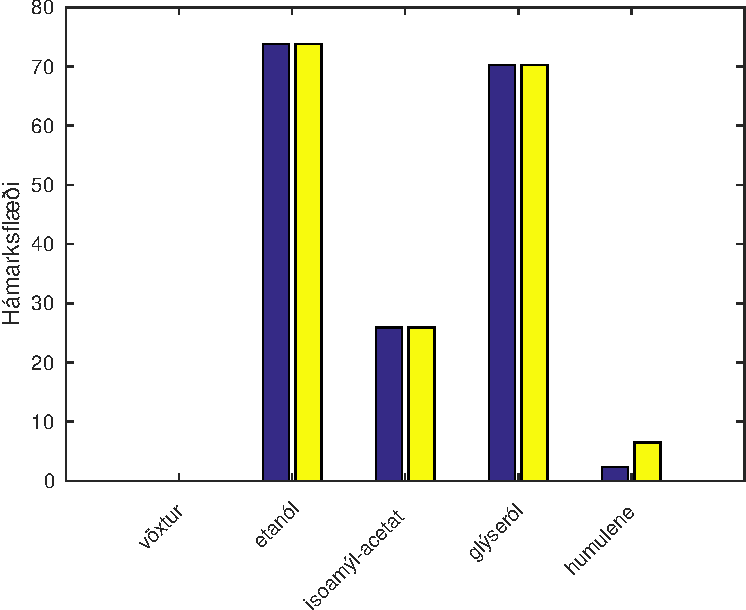
\includegraphics[width=\linewidth]{Pics/BrewingMetMaxFlow}
\end{figureonecolumn}

Þetta er staðfest af þolgreiningu, framleiðsla á humulene reyndist hafa lítil áhrif á hámarksgildi markfalls. Áhrifin á gæðin eru óveruleg sé framleiðsla á humulene ekki þeim mun meiri, eins og sjá má á mynd \ref{fig:robust}. Gæðin liggja vissulega niður á við, en fyrst í stað er hallinn lítill.

\begin{figureonecolumn}
\caption{Áhrif humulene-framleiðslu á markfallsgildi, sem táknar heildargæði bjórsins}
\label{fig:robust}
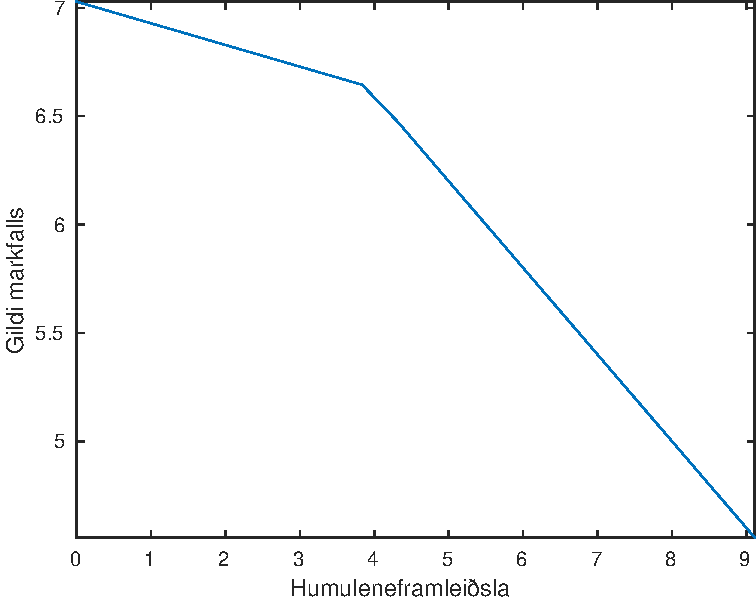
\includegraphics[width=\linewidth]{Pics/BrewingRobustnessAnalysis}
\end{figureonecolumn}
\subsection{Humulene-framleiðsla við sérframleiðsluaðstæður}
Keyrsla OptStrain breytti litlu um heildarafköst gersveppsins við humulene-framleiðslu. Afköstin jukust miðað við óbreytta útgáfu gersveppsins, en þar munaði mest um einfaldara markfall.

GDLS-skrefið ráðlagði útslátt á einu efnahvarfi, \emph{``5-diphosphoinositol-1,2,3,4,6-pentakisphosphate diphosphohydrolase''}, en það dugði ekki til vaxtarkúplunar.
\subsection{Samanburður}
Samanburð á hámarksframleiðslu humulene í óbestuðum gersveppi við bjórgerðaraðstæður og á bestuðum gersveppi við sérhæfðar aðstæður má sjá á mynd \ref{fig:comparative}. Í fyrra tilvikinu er um að ræða hámarksframleiðslu á humulene þegar gildi markfallsins þarf að vera innan 80\% af hámarksgildi sínu, hins vegar einfaldlega hámarksflæði á humulene við bestu fáanlegu aðstæður. Kolefnismagn sem sveppurinn hefur til umráða er í báðum tilvikum það sama.

\begin{figureonecolumn}
\caption{Samanburður á humuleneframleiðslu við bjórgerðaraðstæður og við hámörkunaraðstæður}
\label{fig:comparative}
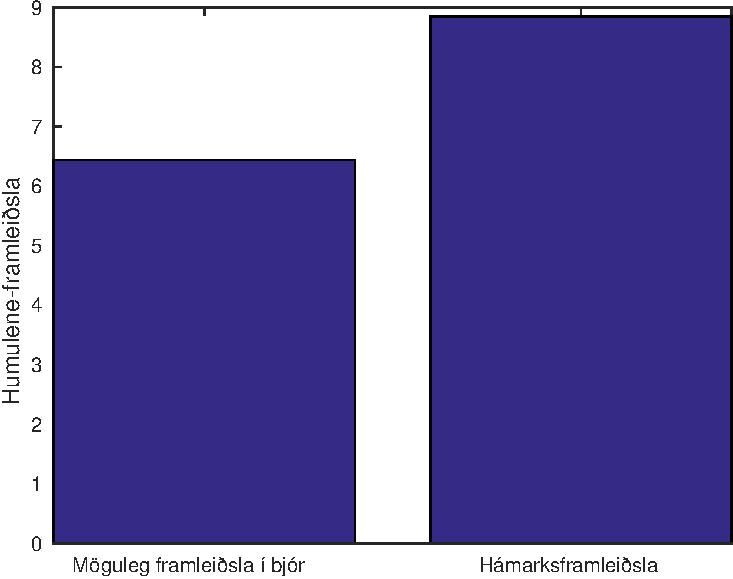
\includegraphics[width=\linewidth]{Pics/ComparativeProduction}
\end{figureonecolumn}

Kolefnisnýtingin til humulene-framleiðslu verður að hámarki $\approx32\%$ í bjórnum, en $\approx44\%$ við sérhæfðu aðstæðurnar.

\section{Ályktanir}
% Byrjar oftast eins: Here we set out to...

% \paragraph{Samantekt á niðurstöðum}
% \paragraph{Hvernig falla niðurstöðurnar að öðrum þekktum niðurstöðum}
% Ræða hvern undirtitil í niðurstöðu-hlutanum sérstaklega
% Aftur samantekt á síðustu málsgreinum, summary of impact

Það magn humulene sem æskilegt væri að láta gersveppinn framleiða er mismunandi eftir bjórtegundum sem brugga skal. Sé framleiðslan á humulene meiri í því afbrigði gersveppsins sem tekst að rækta á rannsóknarstofu heldur en bjór er talinn þurfa mætti nota erfðabreytta gersveppinn í bland við hinn óerfðabreytta.

Í framhaldinu: Skoða Myrcene \cite[KEGG: C06074]{Kanehisa01012000}, sem er mögulega mikilvægasta sesquiterpene-ið þegar kemur að lykt bjórs \cite{guadagni1966odour}. OptForce\cite{ranganathan2010optforce} hefur gefið góða raun í svipuðum verkefnum og mætti prófa í stað OptStrain.

%%%%%%%%%%%%%%
% HEIMILDASKRÁ
%%%%%%%%%%%%%%
\bibliographystyle{plain}
\bibliography{bioinfo.bib}

\end{multicols}

%%%%%%%%%%%%%%
% VIÐAUKI
%%%%%%%%%%%%%%

\clearpage
\appendix
\section{Kóði}
Hér má finna valin kóðadæmi. Allan forritskóða og gögn sem unnið er með má finna á \href{https://github.com/Ernir/optstrain}{Github-síðu verkefnisins}.

\subsection{constructObjectiveFunction.m}
\label{code:constructObjectiveFunction}
\matlab{../constructObjectiveFunction.m}

\subsubsection{enhancedBrewing.m}
\label{code:enhancedBrewing}
\matlab{../enhancedBrewing.m}

\subsection{simpleObjectiveFunction.m}
\label{code:simpleObjectiveFunction}
\matlab{../simpleObjectiveFunction.m}

\subsection{OptStrain.m}
\label{code:OptStrain}
\matlab{../OptStrain.m}

\end{document}